\documentclass[12pt]{article}
\usepackage{HomeWorkTemplate}
\usepackage{circuitikz}
\usepackage{tikz}
\usepackage{float}
\usepackage{mathtools}
\usepackage{xepersian}
\usetikzlibrary{arrows,automata}
\usetikzlibrary{circuits.logic.US}
\settextfont{XB Niloofar}
\newcounter{problemcounter}
\newcounter{subproblemcounter}
\linespread{1.2}
\setcounter{problemcounter}{1}
\setcounter{subproblemcounter}{1}
\newcommand{\grade}[1]{\textbf{(#1 نمره)}}
\newcommand{\problem}[1]
{
\section*{
مسأله‌ی
\arabic{problemcounter} 
\stepcounter{problemcounter}
\setcounter{subproblemcounter}{1}
#1
}
}
\newcommand{\subproblem}{
\subsection*{\alph{subproblemcounter})}\stepcounter{subproblemcounter}
}
\newcommand{\n}{

\null

}
\begin{document}

\handout
{نظریه‌ی زبان‌ها و اتوماتا}
{}
{دانشجو: علیرضا توفیقی محمدی}
{سری 1}
{شماره‌ی دانشجویی: 96100363}


\problem{}
\subproblem{}
% 1.1
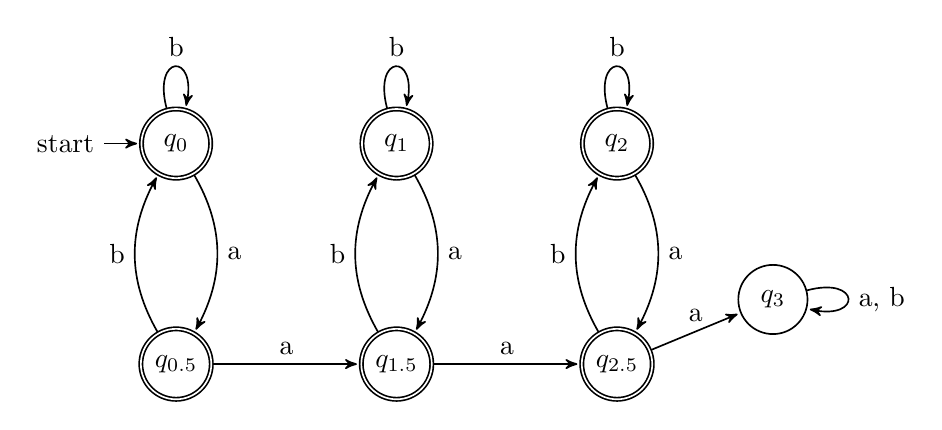
\begin{tikzpicture}[->,>=stealth',shorten >=1pt,auto,node distance=2.8cm,semithick]

\node[initial,state,accepting] (Q0)                {$q_0$};
\node[state,accepting]         (Q05) [below of=Q0] {$q_{0.5}$};
\node[state,accepting]	     (Q1)  [right of=Q0] {$q_{1}$};
\node[state,accepting]         (Q15) [below of=Q1] {$q_{1.5}$};
\node[state,accepting]	     (Q2)  [right of=Q1] {$q_{2}$};
\node[state,accepting]         (Q25) [below of=Q2] {$q_{2.5}$};
\node[state]         (Q3) [below right of=Q2] {$q_{3}$};

\path
(Q0)  edge [loop above] node {b} (Q0)
	  edge [bend left] node {a} (Q05)
(Q05) edge [bend left] node {b} (Q0)
	  edge [above] node {a} (Q15)
(Q1)  edge [loop above] node {b} (Q1)
	  edge [bend left] node {a} (Q15)
(Q15) edge [bend left] node {b} (Q1)
	  edge [above] node {a} (Q25)
(Q2)  edge [loop above] node {b} (Q2)
	  edge [bend left] node {a} (Q25)
(Q25) edge [bend left] node {b} (Q2)
	  edge [above] node {a} (Q3)
(Q3) edge  [loop right] node {a, b} (Q3)
	   
;
\end{tikzpicture}
\subproblem{}
% 1.2
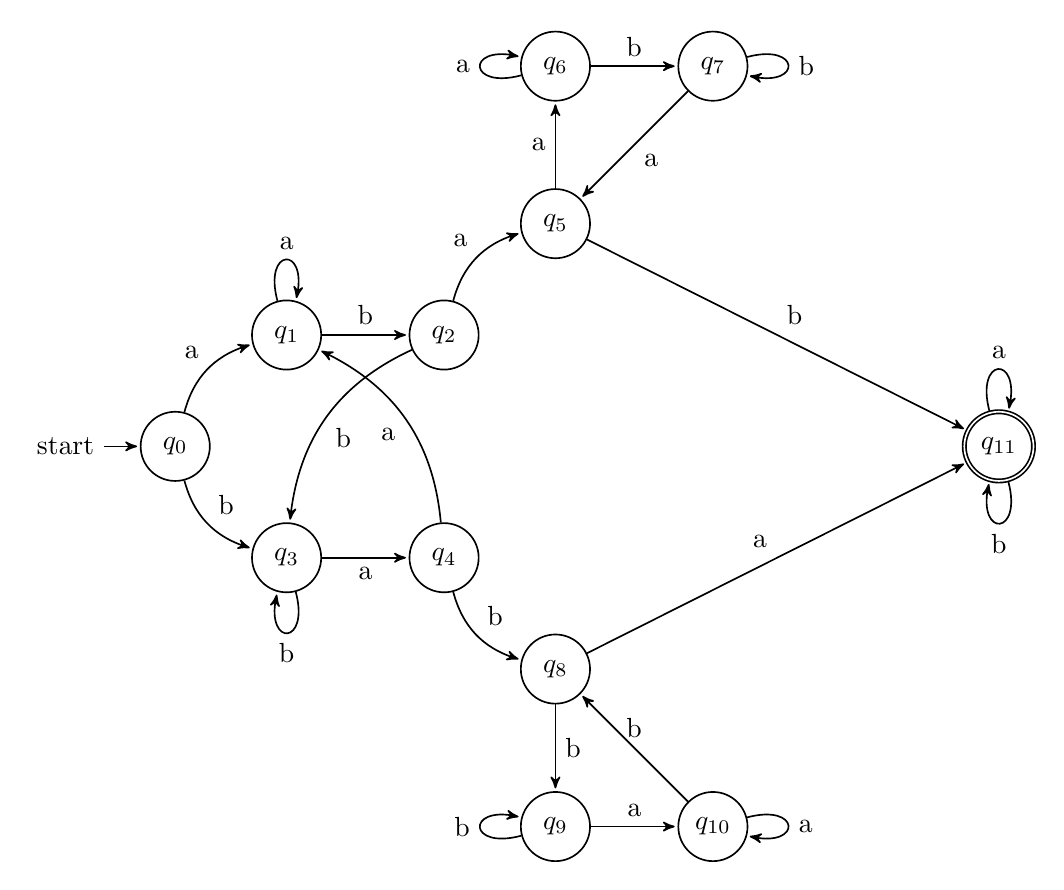
\begin{tikzpicture}[->,>=stealth',shorten >=1pt,auto,node distance=2cm,semithick]

\node[initial,state] (S) {$q_0$};
\node[state] (A00) [above right of=S] {$q_1$};
\node[state] (A01) [right of=A00] {$q_2$};
\node[state] (A10) [below right of=S] {$q_3$};
\node[state] (A11) [right of=A10] {$q_4$};

\node[state] (B0) [above right of=A01] {$q_5$};
\node[state] (B1) [above of=B0] {$q_6$};
\node[state] (B2) [right of=B1] {$q_7$};

\node[state] (C0) [below right of=A11] {$q_8$};
\node[state] (C1) [below of=C0] {$q_9$};
\node[state] (C2) [right of=C1] {$q_{10}$};
\node[state,accepting] (D) [right, xshift=10cm] {$q_{11}$};
\path
(S) edge [bend left] node {a} (A00)
    edge [bend right] node {b} (A10)
(A00) edge [above] node {b} (A01)
      edge [loop above] node {a} (A00)
(A10) edge [below] node {a} (A11)
      edge [loop below] node {b} (A10)
(A01) edge [bend right] node {b} (A10)
      edge [bend left] node {a} (B0)
(A11) edge [bend right] node {a} (A00)
      edge [bend right] node {b} (C0)
(B0) edge [] node {a} (B1)
     edge [] node {b} (D)
(B1) edge [loop left] node {a} (B1)
     edge [] node {b} (B2)
(B2) edge [] node {a} (B0)
     edge [loop right] node {b} (B2)
(C0) edge [] node {b} (C1)
     edge [] node {a} (D)
(C1) edge [loop left] node {b} (C1)
     edge [] node {a} (C2)
(C2) edge [above] node {b} (C0)
     edge [loop right] node {a} (C2)
(D) edge [loop above] node {a} (D)
    edge [loop below] node {b} (D)
;
\end{tikzpicture}

\subproblem{}
% 1.3
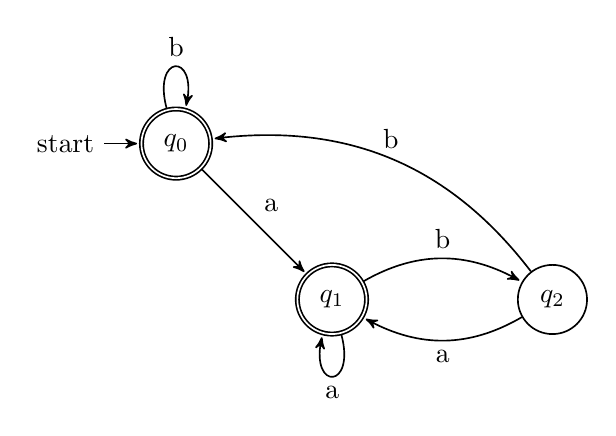
\begin{tikzpicture}[->,>=stealth',shorten >=1pt,auto,node distance=2.8cm,semithick]

\node[initial,state,accepting] (A)                    {$q_0$};
\node[state,accepting]         (B) [below right of=A] {$q_1$};
\node[state]	         	   (C) [right of=B] {$q_2$};

\path
(A) edge [loop above] node {b} (A)
    edge node {a} (B)
(B) edge [loop below] node {a} (B)
	edge [bend left, above] node {b} (C)
(C) edge [bend left, below] node {a} (B)
    edge [bend right, above] node {b} (A)
;
\end{tikzpicture}

\problem{}
\subproblem{}
همه‌ی کلمه‌هایی که شامل زیررشته‌ی $aaba$ باشند.
\subproblem{}
همه‌ی کلمه‌هایی که به رشته‌ی $aaba$ ختم شوند.

\problem{}
\subproblem{}
برای اثبات حالت بندی می‌کنیم. 
\subsubsection*{$m = |S \cap \{0,1,2,3,\dots\}|$ متنهای باشد}
که در این صورت چون 
$|A| \leq m$
و
برای هر زبان متناهی عضوی یک \dfa` داریم که آن‌را بپذیرد پس \dfa ای برای $A$ داریم. (برای اثبات این گزاره کافی‌است یک \dfa به شکل درخت با 
$|\Sigma|^{\max{\{|w| | w \in A\}}} + 2$
حالت رسم کنیم که هر حالت متناظر با یک کلمه‌ی حداکثر 
$\max{\{|w| | w \in A\}}$
حرفی و یک حالت برای کلمات با حرف‌های بیشتر باشد و حالت‌های کلمات متناظر را نهایی بگذاریم)

\subsubsection*{$|S \cap \{0,1,2,3,\dots\}|$ متناهی نباشد}
که در این صورت ادعا می‌کنیم اعداد $n'$ صحیح و نامنفی و $p'$ صحیح و مثبت موجود اند که 
$$S \cap \{0,1,2,3,\dots\} = \{n' + ip' | i \geq 0\}$$
در 
$S = \{n + ip | i \geq 0\}$
باید $p > 0$ باشد، زیرا در غیر اینصورت $n = \max{S}$ و  $S$ متناهی می‌شد، . همچنین چون
$S \cap \{0,1,2,3,\dots\}$
نامتناهی عضوی است، پس تهی نیست و طبق اصل خوش‌ترتیبی در اعداد طبیعی $S$ مینیمم دارد.

حال 
$n' = \min{(S \cap \{0,1,2,3,\dots\})}$
و
$p' = p$
اختیار می‌کنیم.

حال 
$Q = \{q_0, ..., q_{n'+p'}\}$
در نظر بگیرید و تابع $\delta$ را به شکل زیر در نظر بگیرید:
\begin{equation*}
\delta(q_i, a) =
\begin{cases*}
q_{i+1} & if $i < n'+p'$ \\
q_n        & if $i = n' + p'$
\end{cases*}
\end{equation*}
حال \dfa ی
$D$ را به شکل زیر تعریف کنید:
$D = (Q, {a}, \delta, q_0, \{q_n\})$
نسبتا واضح است که $L(D) = A$ پس \dfa ای وجود دارد که $A$ را بپذیرد.

\subproblem{}
ابتدا ادعا می‌کنیم زبان یک \dfa با مجموعه حالت‌های نهایی 
$F = \{f_1, ..., f_k\}$
برابر با اجتماع زبان $k$تا \dfa با مجموعه‌ی الفبا، حالت‌ها و حالت‌اولیه‌ی برابر با \dfa اصلی و حالت نهایی $i$ام برابر با $\{f_i\}$ است.

با توجه به واضح بودن اثبات گزاره‌ی بالا با کمک $\hat{\delta}$ از اثبات آن صرف نظر می‌کنیم و به ادامه‌ی راه حل مسئله می‌پردازیم:

پس تنها کافی‌است گزاره‌ی مسئله را برای \dfa ای با یک حالت نهایی ثابت کنیم. (اگر \dfa ی ما حالت نهایی نداشته‌باشد، در این صورت $A$ تهی بوده و با قراردادن $n = i = -1$ مسئله حل می‌شود.)

فرض کنید $A$ توسط \dfa ی 
$D = (\{q_0,...,q_m\}, {a}, \delta, q_0, \{q_m\})$
پذیرفته شده‌باشد. (بدون خدشه به کلیت مسئله فرض‌کردیم که $Q = \{q_1, ..., q_m\}$ و $F$ تک عضوی و  $F = \{q_m\}$ است. )

حال $\deltaHat$ را برای $D$ می‌سازیم. 


$x_0 = \deltaHat(q_0, \epsilon)$
و
$x_i = \deltaHat(q_0, a^i)$ 
تعریف کنید. 
طبق اصل لانه‌کبوتری و اینکه $|Q| = m$ و $x_i \in Q$ 
در 
$x_0, ..., x_m$
حداقل یک عضو تکراری داریم. اولین $i$ که $x_i \in \{x_0, ..., x_{i-1}\}$ را $k$ بنامید و فرض کنید $x_k = x_j$ که $j < k$.

در این صورت داریم 
$x_{j + r (k-j) + f} = x_{j + f}$

حال اگر 
$q_m \notin \{x_0, ..., x_{k-1}\}$
 که زبان تهی است و یک تصاعد حسابی تهی داریم که در بالا داده شد. و مسئله حل می‌شود.

اگر 
$q_m \in \{x_0, ..., x_{j-1}\}$
که آن‌گاه 
$q_m \notin \{x_{j}, ..., x_k\}$
(زیرا در غیر این‌صورت اولین عضو تکراری $k$ نبود) و در نتیجه زبان تنها شامل یک کلمه است، فرض کنید $q_m = x_t$ و در نتیجه طبق تعریف $x_t$،
$A = \{ a^t\}$
و درنتیجه با قرار دادن $n = t, i = -n-1$ یک تصاعد حسابی با تک عضو $t$ ساخته‌شده و مسئله حل می‌شود.

حال اگر 
$q_m \in \{x_{j}, ..., x_{k-1}\}$
باشد؛ فرض کنید $q_m = x_t$ که $j \leq t < k$ همچنین با توجه به اولین تکرار بودن $k$، هیچ $i$ دیگری که $j \leq i < k$ وجود ندارد که $x_i$ برابر با $q_m$ باشد. پس در این صورت مجموعه‌ی $x_i$ هایی که برابر با $q_m$ اند برابر با
$\{t + (k-j)r| r \in \mathbb{N}\cup\{0\} \}$
است، پس با قرار دادن $n = t$ و $i= (k-j)$ یک تصاعد حسابی به شکل 
$S = \{n + ir | r \in Z \}$
یافت می‌شود و مسئله در این حالت هم حل می‌شود.

پس در حالت یک حالت نهایی با توانستیم $A$ را با یک تصاعد حسابی بسازیم پس در حالتی که $k$ حالت نهایی داریم طبق گزاره‌ی ابتدایی می‌توانیم $A$ را با اجتماع $k$ تصاعد حسابی بسازیم.


\problem{}
% 4
فرض کنید 
$D = (Q, \Sigma, \delta, q_0, F)$
یک \dfa باشد که $L_1$ را بپذیرد، در این صورت $F'$ را به کمک 
$\deltaHat$
 برای $D$ به‌شکل زیر تعریف کنید:
$$F' = \{q | \exists w \in L_2: \deltaHat(q, w) \in F\}$$

حال \dfa ی 
$D' = (Q, \Sigma, \delta, q_0, F')$
را در نظر بگیرید.

با توجه به اینکه فقط حالت‌های نهایی در $D$ و $D'$ متفاوت است درنتیجه $\deltaHat_D = \deltaHat_{D'}$ است.

حال
$L(D') = L_1/L_2$
زیرا:
$$
x \in L(D') \iff \deltaHat_{D'}(q_0, x) \in F' $$$$
\iff \exists y \in L_2: \deltaHat_D(\deltaHat_{D'}(q_0, x), y) \in F $$$$
\iff \exists y \in L_2: \deltaHat_D(\deltaHat_D(q_0, x), y) \in F $$$$
\iff \exists y \in L_2: \deltaHat_D(q_0, xy) \in F $$$$
\iff \exists y \in L_2: xy \in L(D) $$$$
\iff \exists y \in L_2: xy \in L_1 $$$$
x \in L_1/L_2$$

پس $D'$ زبان $L_1/L_2$ را می‌پذیرد و مسئله حل شد.

\problem{}
%5
\begin{definition}
به کلمه‌ای از حروف $a, b$ که هم تعداد $a$ها و هم تعداد $b$ها در آن فرد باشد \textit{جذاب} می‌گوییم.
\end{definition}

\begin{definition}
به کلمه‌ی جذاب $w$ جدایی ناپذیر می‌گوییم اگر هیچ چندتایی از کلمات جذاب $v_1, ..., v_k$ وجود نداشته باشد که $w = v_1 v_2 ... v_k$ و در غیر این‌صورت آن‌را جدایی پذیر می‌نامیم.
\end{definition}

فرض کنید $w$ کلمه‌ای جذاب باشد، می‌توان کلمات جذاب و جدایی‌ناپذیر $v_1, ..., v_k$ را یافت که 
$w = v_1 v_2 ... v_k$
. 
(اثبات به سادگی با افراز متوالی $w$ به کلمات جذاب و با توجه به متناهی بودن طول $w$ واضح است.)

حال واضح است $k$ عددی فرد است زیرا در غیر این‌صورت تعداد $a$ها و $b$ها زوج می‌شد و $w$ جذاب نبود. اگر $R$ عبارتی منظم برای زبان کلمات جذاب جدایی‌ناپذیر باشد، زبان کلمات جذاب با توجه به گزاره‌های بالا،  
$(RR)^*R$
است. (زیرا به تعداد فردی کلمه‌ی جذاب جدایی‌ناپذیر افراز می‌شوند و بالعکس از چسباندن تعداد فردی کلمه‌ی جذاب جدایی ناپذیر یک کلمه‌ی جذاب ساخته می‌شود.)

پس تنها کافی‌است $R$ را بیابیم، در ادامه تلاش می‌کنیم کمی ویژگی برای کلمه‌ی جذاب جدایی‌ناپذیر پیدا کنیم و سپس با کمک آن $R$ را بسازیم.

فرض کنید $v = x_1 x_2 ... x_n$ یک کلمه‌ی جذابِ جدایی‌ناپذیر است و $k$ اولین عددی باشد که کلمه‌ی $x_1 x_2 ... x_k$ جذاب است، اولاً چون $x_1 x_2 ... x_n$ جذاب است، چنین $k$ ای وجود دارد و چون یک کلمه‌ی جذاب حداقل ۲ حرف دارد (حداقل یک \lr{a} و یک \lr{b})، پس $k \geq 2$، همچنین واضح است که $k$ و $n$ زوج‌اند زیرا کلمه‌ی جذاب فرد $a$ و فرد $b$ و در مجموع زوج حرف دارد.

حال سه ویژگی زیر برقرار است:
\begin{enumerate}
	\item $x_k \neq x_{k-1}$:
	زیرا در غیر این‌صورت $x_1 x_2 ... x_{k-2}$ نیز جذاب بود و با کمینه‌بودن $k$ در تناقض بود.
	\item $\forall i \in \mathbb{N}, k+2i \leq n: x_{k+2i-1} = x_{k+2i}$:
	فرض کنید این‌طور نباشد، اولین ‌$i$ ای که 
	$x_{k+2i-1} \neq x_{k+2i}$
	است در نظر بگیرید. حال کلمه‌ی 
	$x_{k+1} x_{k+2} ... x_{k+2i-1}  x_{k+2i}$
	را در نظر بگیرید؛ این کلمه جذاب است زیرا به غیر از دو حرف آخر حرف $2j$ ام و $2j-1$ ام باهم برابرند و تعداد زوجی $a$ و $b$ دارند. و دو حرف آخر یکی $a$ و دیگری $b$ است پس در کل تعداد فردی $a$ و $b$ دارد. از طرفی $x_1 x_2 ... x_k$  نیز جذاب بود، و همچنین $x_1 x_2 ... x_n$ نیز جذاب است. پس 
	$x_{k+2i+1} ... x_n$
	نیز باید جذاب باشد و در نتیجه $v$ جدایی پذیر شد و این تناقض است، پس فرض خلف باطل است و ویژگی دوم نیز ثابت شد.
	\item $\forall i \in \mathbb{N}, 2i < k: x_{2i-1} = x_{2i}$:
	فرض کنید این‌طور نباشد، اولین ‌$i$ ای که 
$x_{2i-1} \neq x_{2i}$
است در نظر بگیرید. حال کلمه‌ی 
$x_{1} x_{2} ... x_{2i-1}  x_{2i}$
را در نظر بگیرید؛ این کلمه جذاب است زیرا به غیر از دو حرف آخر حرف $2j$ ام و $2j-1$ ام باهم برابرند و تعداد زوجی $a$ و $b$ دارند. و دو حرف آخر یکی $a$ و دیگری $b$ است پس در کل تعداد فردی $a$ و $b$ دارد و از طرفی $2i < k$ که با کمینه بودن $k$ در تناقض است.
\end{enumerate}

پس طبق ۳ ویژگی اثبات شده‌ی قبل، $v$ به شکل یک $ab$ یا $ba$ ای است که حروف دو طرف آن به زیر رشته‌های $aa$ و $bb$ افراز می‌شوند.

پس عبارت منظم برای زبان کلمات جذاب جدایی ناپذیر برابر با
$$
R = (aa+bb)^*(ab+ba)(aa+bb)^*
$$
است.

پس عبارت منظم زبان کلمات جذاب برابر با

$$
((aa+bb)^*(ab+ba)(aa+bb)^*(aa+bb)^*(ab+ba)(aa+bb)^*)^*(aa+bb)^*(ab+ba)(aa+bb)^*
$$
است که با کمی ساده‌سازی برابر با
$$
((aa+bb)^*(ab+ba)(aa+bb)^*(ab+ba)(aa+bb)^*)^*(ab+ba)(aa+bb)^*
$$
می‌شود.

حال به ساختن \enfa می‌رسیم...

\problem{}
%6
\subproblem{}
%6.1
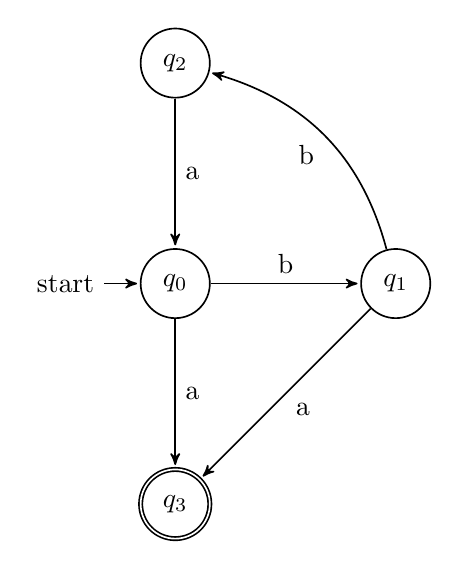
\begin{tikzpicture}[->,>=stealth',shorten >=1pt,auto,node distance=2.8cm,semithick]

\node[initial,state] (A) {$q_0$};
\node[state] (B) [right of=A] {$q_1$};
\node[state] (C)  [above of=A] {$q_2$};
\node[state,accepting] (D) [below of=A] {$q_3$};


\path
(A) edge [] node {b} (B)
    edge [] node {a} (D)
(B) edge [bend right] node {b} (C)
    edge [] node {a} (D)
(C) edge [] node {a} (A);
\end{tikzpicture}

\subproblem{}
% 6.2
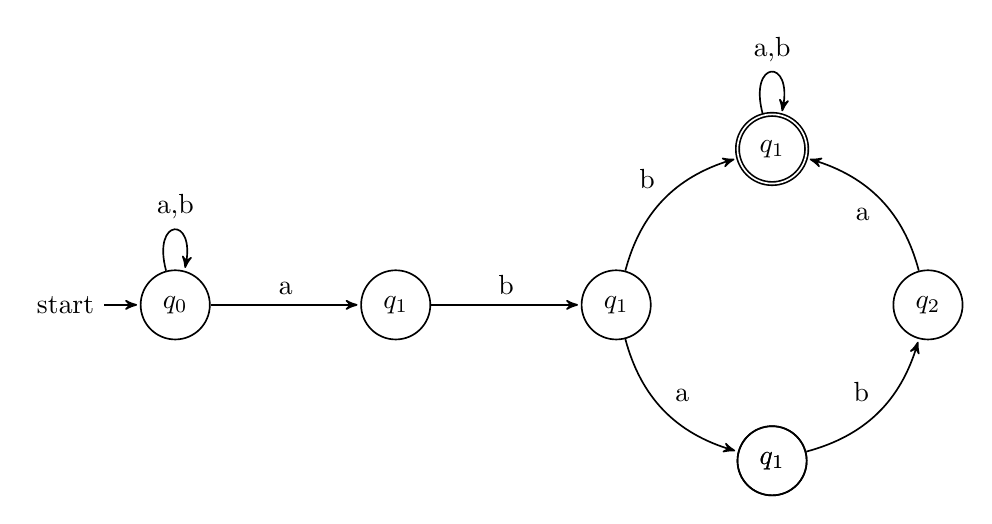
\begin{tikzpicture}[->,>=stealth',shorten >=1pt,auto,node distance=2.8cm,semithick]

\node[initial,state] (A) {$q_0$};
\node[state] (B) [right of=A] {$q_1$};
\node[state] (C) [right of=B] {$q_1$};
\node[state,accepting] (D) [above right of=C] {$q_1$};
\node[state] (E) [below right of=C] {$q_1$};
\node[state] (E) [below right of=C] {$q_1$};
\node[state] (F)  [above right of=E] {$q_2$};


\path
(A) edge [] node {a} (B)
	edge [loop above] node {a,b} (A)
(B) edge [above] node {b} (C)
(C) edge [bend left] node {b} (D)
	edge [bend right] node {a} (E)
(D) edge [loop above] node {a,b} (D)
(E) edge [bend right] node {b} (F)
(F) edge [bend right] node {a} (D)
;
\end{tikzpicture}

\problem{}
کافی است به شکل بازگشتی عمل کنیم؛ دو طرف جمع و کانکت را جا به‌جا کنیم و سپس به شکل بازگشتی عملیات را روی عبارت‌های داخلی انجام دهیم.
$$
abab(bba + ababb)^*
$$

\problem{}
%8
\subproblem{}
% 8.1
$$
\lambda\lambda = \lambda \implies f(\lambda\lambda) = f(\lambda) \implies 
f(\lambda)f(\lambda) = f(\lambda) \implies f(\lambda) = \lambda
$$
\subproblem{}
% 8.2
چون $L$ منظم است پس عبارت منظمی مثل $R$ وجود دارد که $L$ را بپذیرد. حال تابع 
$$g: \Sigma_1 \cup \{(,),+,^*,\emptyset\} \rightarrow \Sigma_2^* \cup \{(,),+,^*,\emptyset\}$$
را در نظر بگیرید که
\begin{equation*}
g(x) =
\begin{cases*}
f(x) & if $x \in \Sigma_1$ \\
x        & otherwise
\end{cases*}
\end{equation*}
حال اگر 
$R = x_1 x_2 ... x_n$
باشد، چون $x_i \in \Sigma_1 \cup \{(,),+,^*\}$، عبارت منظم
$R' = g(x_1) g(x_2) ... g(x_n)$
یک عبارت منظم روی $\Sigma_2$ است که ادعا می‌کنیم زبان آن $F(L)$ است، که اثبات آن به سادگی با کمک استقرا روی تعداد کاراکتر‌های $(,),+,^*,\emptyset$ در $R$ به سادگی به دست می‌آید.

\problem{}
% 9
\subproblem{}
% 9.1
برای اثبات تنها کافی است ثابت کنیم:
$$L^k = L^{k+1} \iff L^k = L^*$$
برای این اثبات از لم‌های زیر استفاده می‌کنم.
\begin{lemma}
\textbf{
اگر $\lambda \in L$ آنگاه 
$L^k \subseteq L^{k+1}$
}.

اثبات نسبتا ساده است، زیرا چون $\lambda \in L$ پس 
$L = \lambda + L$
و در نتیجه:
$$L^{k+1} = L^k L = L^k (\lambda + L) = L^k \lambda + L^kL = L^k + L^kL$$
و در نتیجه $L^k \subseteq L^{k+1}$ و حکم ثابت شد.
\end{lemma}

\begin{lemma}
\textbf{
اگر $L$ یک زبان منظم ناتهی باشد و یکی از دو شرط 
$L^k = L^{k+1}$ یا  $L^k = L^*$
برقرار باشد، آن‌گاه $\lambda \in L$.
}

برای اثبات چون $L$ ناتهی است، پس کلمه‌ای با کمترین طول دارد، کمترین طول را $l$ در نظر بگیرید. کمترین طول در $L^k$ برابر با $lk$ و در $L^{k+1}$ برابر با $l(k+1)$ است و در $L^*$ برابر با ۰ است.

اگر حکم اول برقرار باشد آن‌گاه $lk = l(k+1) \implies l = 0$ و اگر حکم دوم برقرار باشد $lk = 0 \implies l = 0$ (زیرا اگر $k$ صفر باشد آنگاه $L^*$ برابر با $L^0$ یعنی تک رشته‌ی $\lambda$ می‌شود و چون $L$ تهی نیست، مجبور است فقط $\lambda$ را داشته باشد و کمترین طول آن ۰ می‌شود.) پس لم ثابت شد.
\end{lemma}

حال اگر $L = \emptyset$ که $k=0$ هر دو حکم بالا برقرار می‌شود و این $k$ کوچکترین است و گزاره ثابت می‌شود. در ادامه فرض می‌کنیم $L \neq \emptyset$.

\textbf{
اگر $L^k = L^{k+1}$
}\\
اولا واضح است که $L^k \subseteq L^*$. طبق دیگر را ثابت می‌کنیم:
در این صورت برای هر $i$ نامنفی داریم 
$L^{k+i} \subseteq L^{k+i+1}$
و در نتیجه $L^k = L^{k+i}$
همچنین طبق لم۲، $\lambda \in L$ و در نتیجه طبق لم۱ داریم:
$$L^0 \subseteq L^1$$
$$L^1 \subseteq L^2$$
$$L^2 \subseteq L^3$$
...
$$L^{k-1} \subseteq L^{k}$$
و در نتیجه 
$$L^0 \cup L^1 \cup ... \cup L^k \subseteq L^k$$
و در نتیجه 
$$L^0 \cup L^1 \cup ... \cup L^k\cup L^k\cup...\cup L^k \subseteq L^k$$
و در نتیجه 
$$L^0 \cup L^1 \cup ... \subseteq L^k$$
و در نتیجه
$$L^* \subseteq L^k$$

پس $L^* = L^k$.
\\\\
\textbf{
حال اگر $L^k = L^*$.
}\\
اولا که چون $L^{k+1} \subseteq L^{*}$ طبق فرض $L^{k+1} \subseteq L^*$ 

از طرفی طبق لم ۲، $\lambda \in L$ و درنتیجه طبق لم ۱، $L^k \subseteq L^{k+1}$

در نتیجه $L^k = L^{k+1}$.

\subproblem{}
برای پیدا کردن رتبه کافی است $L^0, L^1, ..., L^4$ را در این حالت خاص محاسبه کنیم.
$$L^0 = \{a^k | k = 0 \}$$
$$L^1 = \{a^k | (k = 0) \vee (k \mod 3 = 2) \}$$
$$L^2 = \{a^k | (k = 0) \vee (k \mod 3 = 2) \vee (k > 3 \wedge k \mod 3 = 1) \}$$
$$L^3 = \{a^k | (k = 0) \vee (k \mod 3 = 2) \vee (k > 3) \}$$
$$L^4 = \{a^k | (k = 0) \vee (k \mod 3 = 2) \vee (k > 3) \}$$
پس اولین $k$ ای که $L^k = L^{k+1}$ است، $k=3$ است و رتبه‌ی این زبان ۳ است.

\problem{}
\subproblem{}
%9.1
\subproblem{}
%9.2

$$
(a+b)a^* + (a+b)a^*b(aa*b + b(a+b)a*b)^*(aa*+b(a+b)a^)
$$
\subproblem{}
%9.3
$$
(a+b)(((a+b)(a+b)b)^*(\epsilon+(a+b)(a+b)a(a+b)))^* (\epsilon + (a+b))
$$
\subproblem{}
%9.4
$$
(b + a (ba^*bb)^*(a+ba^*ba))^*
$$
\end{document}
